\begin{marginfigure}[8cm] %MARGIN FIGURE
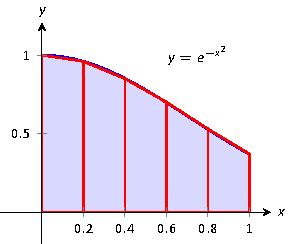
\includegraphics{figures/fignum3a} %Example 134 APEX
\caption{Approximating $\int_0^1 e^{-x^2}\ dx$ using 5 trapezoids of equal widths.}
\label{F:5-6-EG2}
\end{marginfigure}

\begin{margintable} %MARGIN TABLE
\begin{center}
\caption{A table of values of $e^{-x^2}$.} 
\label{T:5-6-EG2} 
\begin{tabular}{cc}
$x_i$ & $e^{-x_i^2}$ \\ \hline
$0$ & 1\\
$0.2$ & $0.961$ \\
$0.4$ & $0.852$ \\
$0.6$ & $0.698$ \\
$0.8$ & $0.527$ \\
$1$ & $0.368$
\end{tabular}
\end{center}
\end{margintable}


\begin{example} \label{eg:5.6.2} % EXAMPLE
Use $5$ trapezoids of equal width to approximate $\ds \int_0^1e^{-x^2}\ dx$.

\solution To compute the areas of the $5$ trapezoids in Figure \ref{F:5-6-EG2}, it will again be useful to create a table of values as shown in Table \ref{T:5-6-EG2}. The leftmost trapezoid has legs of length $1$ and $0.961$ and a height of $0.2$. Thus, by our formula, the area of the leftmost trapezoid is: 
$$ \frac{1+0.961}{2}(0.2) = 0.1961.$$
Moving right, the next trapezoid has legs of length $0.961$ and $0.852$ and a height of $0.2$. Thus its area is: $$\frac{0.961+0.852}2(0.2) = 0.1813.$$

The sum of the areas of all $5$ trapezoids is:
\begin{align*}
\frac{1+0.961}{2}(0.2) + \frac{0.961+0.852}2(0.2)+\frac{0.852+0.698}2(0.2)&+ \\
\frac{0.698+0.527}2(0.2)+\frac{0.527+0.368}2(0.2)&= 0.7445.
\end{align*}

Alternatively, if we use the Trapezoid Rule with $n=5$ along with the results from Example~\ref{eg:5.6.1}, we have
\[ T_5  =  \frac{1}{2}\Big[L_5 + R_5 \Big] \approx \frac{1}{2}\Big[ 0.808 + 0.681 \Big] \approx 0.7445 \]
We approximate $\ds \int_0^1 e^{-x^2}\ dx \approx 0.7445.$
\end{example}

